\chapter{Fast One-Ring Smoothing}
\label{ch4}
In this chapter we present an updated version of \Forf{t}, based on the filter initially proposed by H. Mara and S. Krömker at the EUROGRAPHICS Workshop on Graphics and Cultural Heritage (2017) ~\cite[s.~3.2]{Mara17}. Since publication, further research has been conducted by the authors, and it was determined that improving the weighting methods was possible, therefore, modifcations to the algorithm were implemented directly within the GigaMesh \todoCitation{GigaMesh} framework. This chapter presents the as-yet-unpublished version of \forf{t} as it exists now, with more accuracte weighting based on the interpolation of function values to the center of gravity for each circular sector comprising the geodesic disc centered upon a vertex in a mesh.

%
%
%
%
\section{A Mesh of \tdd{}}
\label{ch4sPE}
Given the triangle mesh of \tdd{} $\bM$, a superset of both a set of points $\bP$ and a set of faces $\bT$, the procedure for \forf{t}  begins by choosing a point $\bp_v$, which defines the one-ring neighborhood $\bN_v$, then calculating the shortest edge length $\elm$ among all the points $\bp_i$ adjacent to the center point $\bp_v$, which  is indexed locally within the neighborhood as $\bp_0$. That shortest edge length
%
\begin{equation}
	\elm(\bp_0) := \text{min}^{|\bN_v|}_{i=1}\,\big(|\bp_i - \bp_0|\big)
	\label{eq:localMinimumEdgeLength}
\end{equation}%
\nomenclature[ba]{$\elm(\bp_v)$}{the shortest edge length in $\bN_v$}%
\nomenclature[ba]{$\bp_0$}{the center point of $\bN_v$}%
%
when considered as a radius, defines the geodesic circle $\bO_v$ about the point $\bv$.

Furthermore, to ensure that the filter window remains the same size\footnote{a footnote about filter window size importance}\todoReword{footnote about filter window size importance}\todoCitation{SBN-13: 9781598296204}\todoResearch{call to question the importance of global minimum edge length in light of the typo found in source} for the entirity of the mesh, we define
%
\begin{equation}
	\gelm := \min\left \{\elm(\bp_0) \;|\; \bp_0 \in \bM\,\right \}
	\label{eq:globalMinimumEdgeLength}
\end{equation}%
\nomenclature[bb]{$\gelm$}{the shortest edge length in $\bM$}%
%   
as the shortest edge length among all adjacent points in the mesh $\bM$, so that in lieu of $\elm$, we can use $\gelm$ in all the following computations presented in this chapter.

Figure~\ref{fig:geodesicDisc} shows a typical configuration of a one-ring neighborhood with irregular faces, the geodesic disc $\bO$ with radius $\elm$, and the circular sectors $\bs_i$.

\begin{figure}[ht]
\ffigbox
	{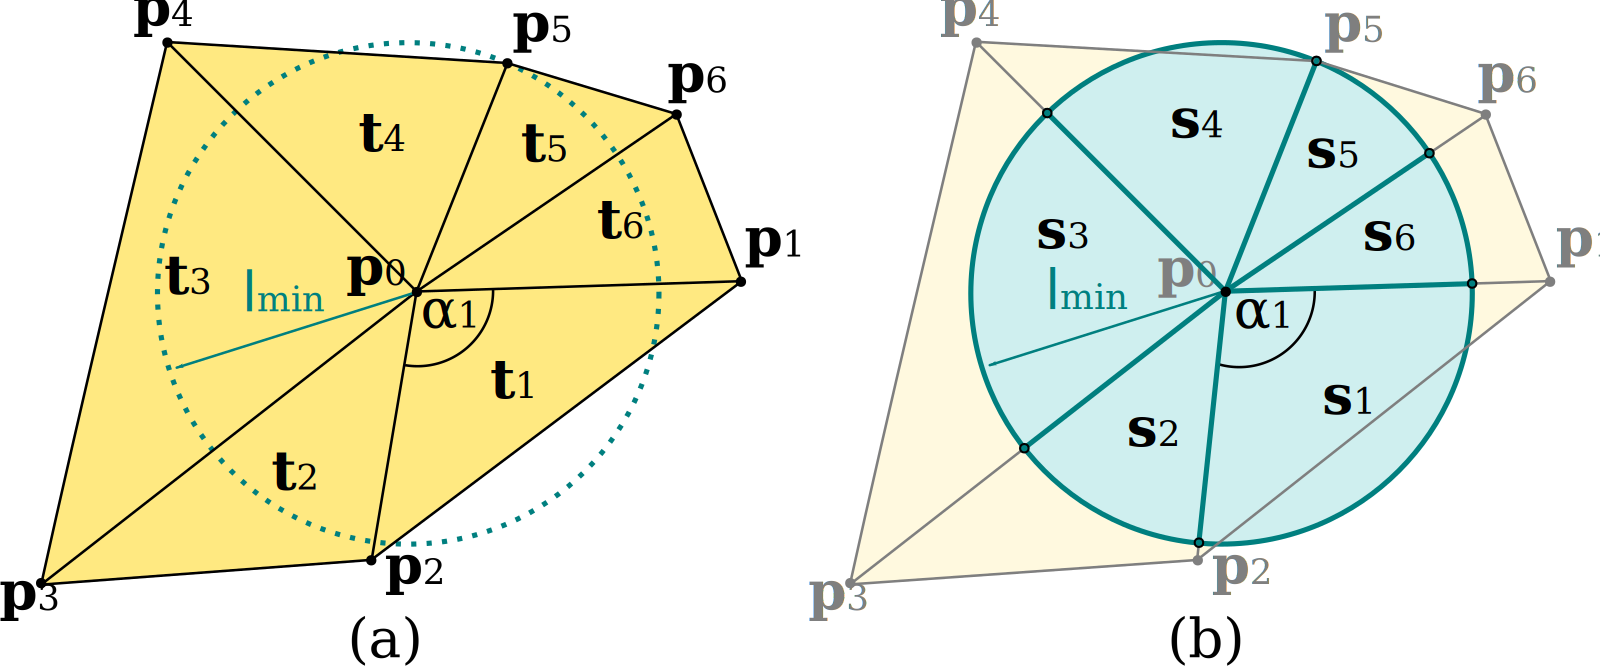
\includegraphics[width=1.0\linewidth]{figures/geodesicDisc.png}}
	{\caption[One-ring and geodesic disc]{A typical one-ring neighborhood $\bN$ with (a) irregular triangular faces $\bt_i$, the smallest edge length $\elm = \ell_4 = |\bp_4 - \bp_0|$ illustrated with a teal arrow as the radius of the geodesic disc, and $\alpha_1$ as the central angle of $\bt_1$ (b) the complete geodesic disc $\bO$, comprised of all its circular sectors $\bs_i$}\label{fig:geodesicDisc}}
\end{figure}%

%
%
%
%
\section{Angles}
\label{ch4sA}
Before we can calculate the area of the circle sectors in $\bO_v$, we must first compute the inner angles $\alpha_i$ for each triangle $\bt_i$ in the neighborhood $\bN_v$. That is possible using the using the Law of Cosines~\cite{Weisstein19e}
%
\begin{equation}
	\alpha_i = cos^{-1}(\frac{|\bp_0 - \bp_{i}|^2 + |\bp_0 - \bp_{\sipo}|^2 - |\bp_i - \bp_{\sipo}|^2}{2\cdot|\bp_0 - \bp_{i}|\cdot|\bp_0 - \bp_{\sipo}|})
\end{equation}
%
or more compactly:
%
\begin{equation}
	\alpha = cos^{-1}\left (\frac{\ell_c^2 + \ell_b^2 - \ell_a^2}{2\cdot\ell_c\cdot\ell_b}\right )
	\label{eq:alphaFromEdgeLengths}
\end{equation}%
\nomenclature[ca]{$\alpha$}{the central angle of a circle sector $\bs$}%

In order to interpolate the function values from each point over the entire sector, we must first interpolate the values one side of the bisecting line at a time, as will be discussed in detail in Section~\ref{ch4sWM}. For those coupled computations, the angles $\beta_i$ will be required, and having now obtained the $\alpha_i$, they can be calculated using a proxy right triangle and the third angle theorem\footnote{otherwise known as the Angle-Angle-Angle Theorem, abbreviated as AAA}~\cite{Weisstein19f} as
%
\begin{equation}
	\beta_i = \Big(\frac{\pi}{2} - \frac{\alpha_i}{2}\Big) = \frac{(\pi - \alpha_i)}{2}
	\label{eq:betaFromHalfAlpha}
\end{equation}%
\nomenclature[cb]{$\beta_i$}{the third angle with $\frac{\alpha_i}{2}$ and $\frac{\pi}{2}$}%

Figure~\ref{fig:anglesAndCenterOfGravity} extends Figure~\ref{fig:geodesicDisc} by enhancing the circle sector $\bs_1$ to show an example of the angles $\alpha/2$ and $\beta$, with the proxy right triangles used to calculate it, as well as the center of gravity which is discussed in detail in Section~\ref{ch4sACG}.

%
%
%
%
\section{Area \& Center of Gravity}
\label{ch4sACG}
Because a circle sector may be described entirely by its radius and central angle~\cite{Weisstein19d}, having now calculated $\gelm$ and $\alpha_i$, the area of the sector can be obtained using the formula
%
\begin{equation}
	A_i = \frac{(\gelm)^2\alpha_i}{2}
	\label{eq:circularSectorArea}
\end{equation}
%
and similarly $\check{\ell}$, the distance from the center point $\bp_0$ along the bisecting line to the center of gravity $\bc_i$ can be calculated directly using the formula
%
\begin{equation}
	\check{\ell} := \frac{4\:\gelm\:\sin(\frac{\alpha_i}{2})}{3\,\alpha_i}
	\label{eq:distToCoG}
\end{equation}%

Figure~\ref{fig:anglesAndCenterOfGravity} extends Figure~\ref{fig:geodesicDisc} by enhancing the circle sector $\bs_1$ to illustrate the center of gravity $\bc$ and its distance from the center point $\bp_0$. In general, while holding the radius constant, the smaller the angle $\alpha$ becomes, the longer the distance $\check{\ell}$ becomes.

\begin{figure}[ht]
\ffigbox
	{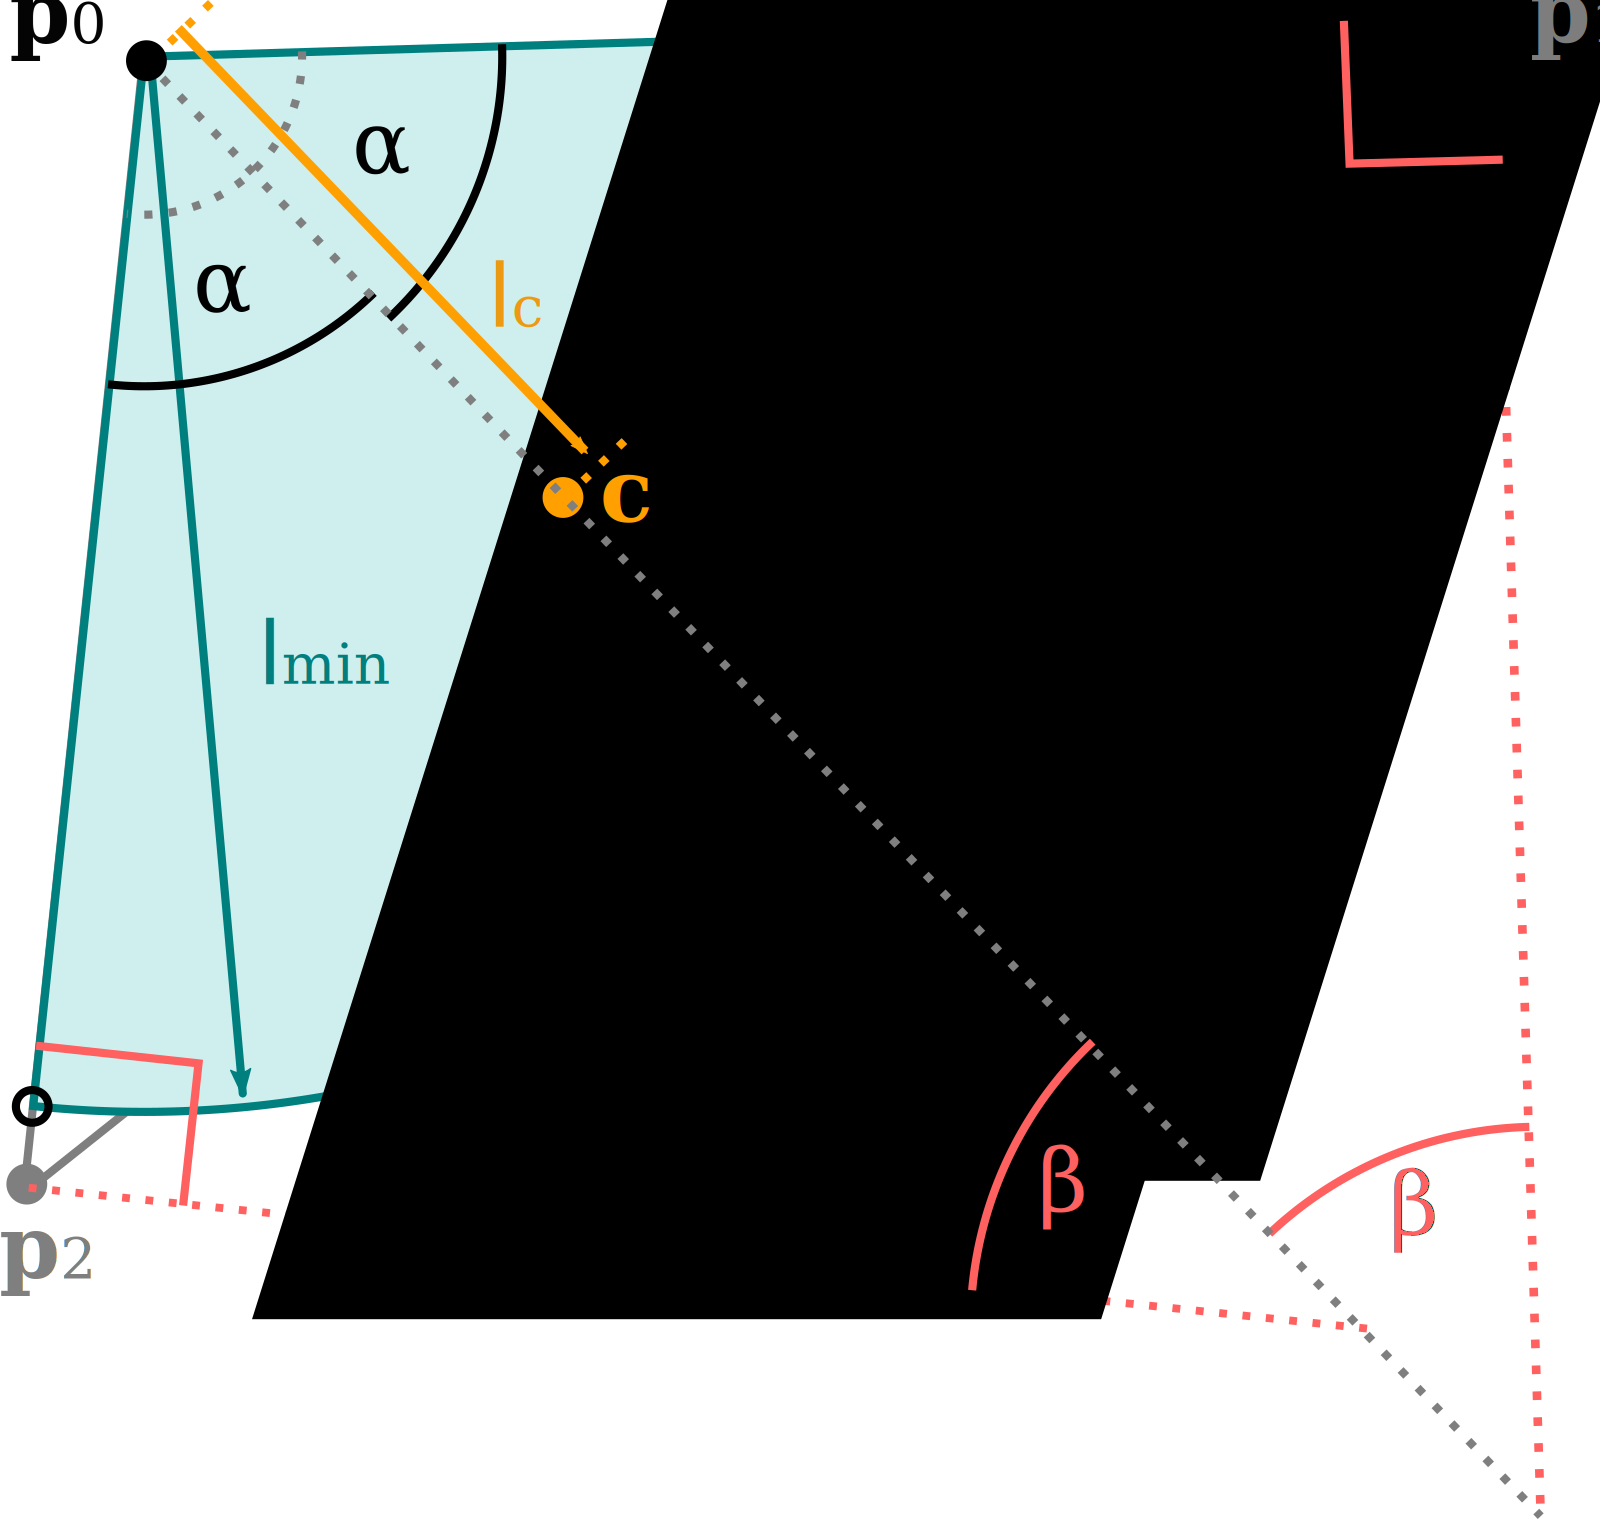
\includegraphics[width=0.5\linewidth]{figures/anglesAndCenterOfGravity.png}}
	{\caption[Angles and Center of Gravity]{An enhanced view of Figure~\ref{fig:geodesicDisc}, focusing on the circle sector $\bs_1$, showing $\alpha$ and the bisecting line in gray dots. In sand color is the center of gravity $\bc$ and $\check{\ell}$, the distance to it from $\bp_0$ along the bisecting line. Also shown in coral color, are the angles $\beta$, with the proxy right triangles used to calculate them.}\label{fig:anglesAndCenterOfGravity}}
\end{figure}%

%
%
%
%
%
\section{Interpolation \& Function Values}
\label{ch4sIFV}
%
\forf{T} is agnostic to the meaning of information represented by the data, therefore, it can similarly process any such function values stored as a scalar field. However, because the filter was designed to only convolve scalar fields, any multi-dimensional data, such as RGB color, must be processed individually as independent scalar fields. The result is that we can define a scalar field simply as a set of function values.
\todoReword{MOVE ME}

The intuition about the importance of , is that any number of triangles which share the same three angles are similar to eachother. In this case, both sides of the bisecting line share $\alpha/2$, $\pi/2$, and $\beta$, so we can exploit that similarity in order to interpolate the function values, a topic discussed in detail in Section:~\ref{ch4sSIssIFV}.
\todoReword{MOVE ME}

Given the scalar field of function values $\bF$, and having now calculated $\beta_i$, and $\gelm$, both values which are constant between halves of the circle sector, we can next use the Law of Sines~\cite{Weisstein19g} to obtain the constant ratio by which we will interpolate the three function values $f_0$, $f_j$, and $f_{\sjpo}$, from the points $\bp_0$, $\bp_j$, and $\bp_{\sjpo}$, toward the center of gravity $\bc_i$. With this ratio
%
\begin{equation}
	\zeta_i = \frac{\gelm}{\sin(\beta_i)}
	\label{eq:zeta}
\end{equation}%
\nomenclature[ea]{$\zeta_i$}{constant ratio for interpolation derived from Law of Sines}%
%
we can obtain both of the distances required to interpolate $f_i$ and $f_{\sipo}$. 

It should be noted that because the points $\bp_i$ and $\bp_{\sipo}$ are likely at different distances from the center point $\bp_0$, we must now begin calculating for each half of the circular sector individually. One may look to Figures~\ref{fig:geodesicDisc} and~\ref{fig:centerOfGravity} for an example. Therefore, while subscript for $\zeta_i$ remains the match of index for the circle sector $\bs_i$, we will now adopt the subscipt for $\Dz_i$ to denote the side of the sector defined by its point $\bp_i$, also with $\Dz_{\sipo}$ for $\bp_{\sipo}$.
\begin{align}
	\Dz_i & = \kern4pt\frac{\zeta_i}{|\bp_0 - \bp_i|}
	\label{eq:distanceIForInterpolation}\\
	\Dz_{\sipo} & = \frac{\zeta_i}{|\bp_0 - \bp_{\sipo}|}
	\label{eq:distanceIp1ForInterpolation}
\end{align}%
\nomenclature[eb]{$\Dz^i_i$}{also $\Dz^i_{\sipo}$, the distances for interpolation of $f_i$ toward $f_0$}%

From the original function values $f_0$, $f_i$, and $f_{\sipo}$, we can now interpolate based on their distances $\Dz_i$ and $\Dz_{\sipo}$, to become
\begin{align}
	f'_i & = f_0(1 - \Dz_i) + f_i\Dz_i
	\label{eq:interpolatedFi} \\
	f'_{\sipo} & = f_0(1 - \Dz_{\sipo}) + f_{\sipo}\Dz_{\sipo}
	\label{eq:interpolatedFip1}
\end{align}%
\nomenclature[ec]{$f'_i$}{also $f'_{\sipo}$, the interpolated values of $f_i$ toward $f_0$}%

Figure~\ref{fig:interpolation} illustrates the\dots
\begin{figure}[ht]
\ffigbox
	{\includegraphics[width=0.6\linewidth]{example-image-16x9.png}}
	{\caption[Interpolation of Function Values toward the Centroid]{Interpolation of Function Values toward the Centroid\ldots}\label{fig:interpolation}}
\end{figure}

%
%
%
%
\section{Weighted Mean}
\label{ch4sWM}
To calculate the weighted mean function value $f^\bs_i$ at the center of gravity $\bc_i$ of the circle sector $\bs_i$, we must use $f_0$, the function value at $\bp_0$, both interpolated function values, $f'_i$ and $f'_{\sipo}$, and the distance to the center of gravity $\Dc_i$, and we obtain
\begin{equation}
	f^\bs_i = f_0(1 - \Dc_i) + \frac{(f'_i + f'_{\sipo})\Dc_i}{2}
	\label{eq:weightedMeanAtCoGatSector}
\end{equation}%
\nomenclature[fa]{$f^\bs_i$}{the weighted mean function value at $\bc_i$ of $\bs_i$}%

Finally, we can compute the one-ring weighted mean function value at $\bp_0$ by summing all the weighted mean function values from each $\bs_i$ in $\bN$, weighting those again by each sector's area $A_i$, then finally dividing by the total area of the geodesic disc.
\begin{equation}
	\bar{f}_0 := \frac{\sum A_if^{\bs}_i}{\sum A_i} \quad \forall i \in \{1,\ldots,|\bt_v|\}
	\label{eq:meanFuncValAtP0}
\end{equation}%
\nomenclature[fb]{$\bar{f}_0$}{the one-ring weighted mean function value at $\bp_0$}%

The one-ring smoothing filter can be modified to use the median operation, instead of the mean, by using all the equations except Equation~\ref{eq:meanFuncValAtP0} and then sorting the results of Equation~\ref{eq:weightedMeanAtCoGatSector}. The details of which can be found by the original publication ~\cite[s.~3.2]{Mara17}, but as it was not implemented in GPGPU for this thesis, we exclude the details here.

Figure~\ref{fig:weightedMean} illustrates the\dots
\begin{figure}[ht]
\ffigbox
	{\includegraphics[width=0.6\linewidth]{example-image-16x9.png}}
	{\caption[Weighted Mean function value $f^\bs_i$ at the center of gravity]{the weighted mean function value $f^\bs_i$ at the center of gravity\ldots 3D circle sector as base, floating plane above tilted be interpolated function values, area underneath colored.}\label{fig:weightedMean}}
\end{figure}
%
\section{Summary}
\label{ch4sS}
In this chapter we presented an updated version of the Fast One-Ring smoothing filter for scalar fields on discrete manifolds, which since its original publication ~\cite[s.~3.2]{Mara17}, now utilizes the entire area of the geodesic discs centered at $\bp_0$ to calculate the weighted averages of the function values in its one-ring neighborhood. First, we have illustrated how one can calculate the global smallest edge length $\gelm$, interior angles $\alpha$ and $\beta$, the area $A$ of a sector $\bs$ from the geodesic disc $\bO$, and distance $\Dc$ to the centroid (center of gravity) $\bc$ for any given one-ring neighborhood $\bN$ of mesh $\bM$. Next, we provided the equations for interpolating the three function values $f_0$, $f_i$, and $f_{\sipo}$ using the sectorially-constant ratio $\zeta$ to obtain the weighted mean function value for each $\bs$, and finally the weighted mean function value $\bar{f_0}$ at point ${\bp_0}$ for the entire one-ring neighborhood $\bN$. Convolving this filter with the scalar field of function values at each vertex in a mesh for any number of iterations, thus produces a smoothing effect with increasing intensity in relation to the number of iterations.
